\subsection{3D Engine}
\label{sec:3d-engine}
\writer{Albert}

The 3D Engine is the component of the application that handles the animation of objects and displays it on the screen for the user. Its main functions are: 

\begin{itemize}
\item handling the window in which the graphical simulation is shown to the user
\item take care of the user interactions with the window buttons (\textit{Play, Pause, Stop}).
\item take care of the user inputs in the case of \textit{Input Places}
\item draw the graphical objects
\item maintain the communication with the \textit{Simulator}
\item update the animations according to the information sent by the \textit{Simulator}
\end{itemize}

In order to build a system that is not technology dependent in terms of its 3D visualization, Interfaces and the Factory design pattern are employed. In this way, the 3D Engine can be easily changed from \textbf{jMonkey} to \textbf{Java3D} or any other technology desired at some point by the customer. 

Figure \ref{fig:factory} shows the defined classes in the implementation of the Factory pattern.

\begin{figure}[htp]
\begin{center}
  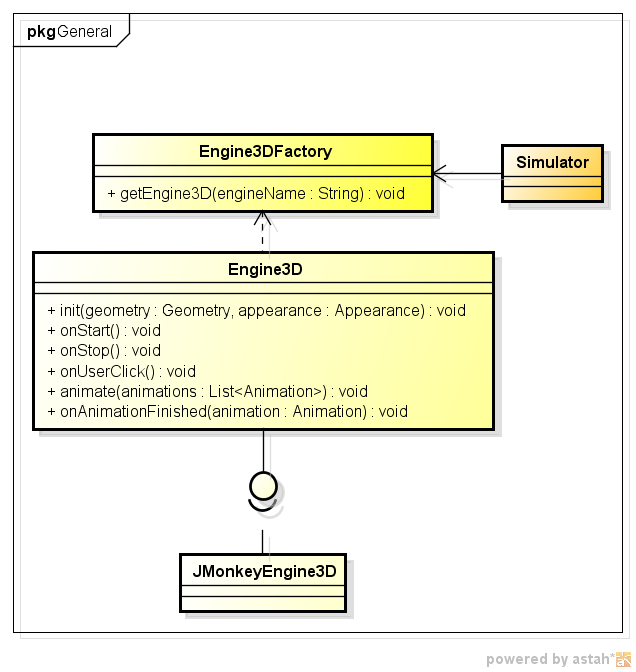
\includegraphics[width=0.8\textwidth]{image/engine_factory.png}
  \caption{3D Engine Factory Pattern}
  \label{fig:factory}
\end{center}
\end{figure} 

\paragraph{Engine3DFactory}

The Engine3DFactory class will be in charge of creating 3D Engine classes according to the engine name sent as a parameter of the method \textit{getEngine3D()}. This method will be called from the Simulator in the initialization phase, when both the 3D Engine and the Petri net Engine are created. 

\paragraph{Engine3D}

Engine3D is an Interface which will be implemented by the actual 3D Engine of the applicaton, in our case \textbf{JMonkeyEngine}. The following methods will be provided by the Engine3D interface: 
\begin{itemize}
\item \textit{init(Geometry geometry, Appearance appearance)} - used to initialize the geometry and appearance models;
\item \textit{startAnimation(List<Animation> animations} - used by the Simulator to send the list of animations to be performed by the 3D Engine; 
\end{itemize}

\paragraph{JMonkeyEngine3D}

As stated before, the JMonkeyEngine3D class will implement all the methods of the Engine3D interface and will perform all the animations. This class will be described into more details in the next section.